\documentclass[10pt,a4paper]{article}

% Rapport scientifique coEnergy : version finale
\usepackage[utf8]{inputenc}
\usepackage[T1]{fontenc}
\usepackage[french]{babel}
\usepackage{lmodern}
\usepackage{microtype}
\usepackage[a4paper,top=2.25cm,bottom=2.2cm,left=2.35cm,right=2.35cm]{geometry}
\usepackage{amsmath,amssymb}
\usepackage{graphicx}
\usepackage{booktabs}
\usepackage{array}
\usepackage{caption}
\usepackage{subcaption}
\usepackage{hyperref}
\usepackage{enumitem}
\usepackage{placeins}
\usepackage{float}
\usepackage{multirow}
\usepackage{setspace}

\hypersetup{hidelinks}
\setstretch{1.045}
\setlength{\parindent}{0pt}
\setlength{\parskip}{0.40em}
\captionsetup{font=small,labelfont=bf}
\setlist[itemize]{topsep=0.25em,itemsep=0.1em,leftmargin=*}
\renewcommand{\arraystretch}{1.16}
\graphicspath{{figures/}}
\newcommand{\hlc}{\mathrm{HLC}}
\newcommand{\hlcext}{\mathrm{HLCext}}
\newcommand{\hlcmit}{\mathrm{HLCmit}}
\newcommand{\taub}{\tau_b}
\newcommand{\taun}{\tau_n}
\newcommand{\tauinf}{\tau_{\infty}}

\title{\textbf{Identification des propriétés thermiques des bâtiments}\\[0.4em]
       \large Étude comparative de réseaux de neurones sur données simulées}
\author{Projet coEnergy}
\date{Novembre 2026}

\begin{document}
\maketitle
\vspace{-1.4em}
\begin{abstract}
J'ai étudié l'identification de six paramètres thermiques d'un bâtiment à partir des séries de température intérieure et de sollicitation. Après des essais \textbf{préliminaires sur 500\,000 simulations}, j'ai comparé six configurations sur \textbf{1\,000\,000 simulations}, avec les mêmes partitions d'entraînement et de test. Le meilleur modèle de cette campagne est une \textbf{fusion CNN--GRU + MLP}, entraînée avec une perte équilibrée entre déperditions thermiques et constantes de temps. Sur le test principal de 89\,987 simulations, elle atteint notamment $R^2=0{,}4911$ pour HLCext, $0{,}4442$ pour HLC et $0{,}2734$ pour $\tau_n$. J'ai également testé une perte donnant davantage de poids aux constantes de temps (30/70), sans obtenir d'amélioration. Ce rapport explique mes choix, les résultats obtenus et les limites rencontrées, notamment pour les constantes de temps. J'ai enfin imposé la relation physique $\mathrm{HLC}=\mathrm{HLCext}+\mathrm{HLCmit}$ en prédisant cinq paramètres indépendants plutôt que six valeurs sans contrainte.

\end{abstract}

\vspace{-0.25em}
\tableofcontents
\vspace{0.5em}
\noindent\textbf{Périmètre.} Je distingue deux étapes : les essais \emph{préliminaires} réalisés sur 500\,000 simulations, puis les six derniers entraînements sur un million. Les derniers runs ne représentent donc pas toutes les expérimentations du projet. Les résultats finaux sont issus des métriques sauvegardées dans les archives Kaggle.

\section{Introduction et objectif scientifique}

\subsection{Un problème inverse de caractérisation thermique}
Dans ce travail, j'ai cherché à estimer les propriétés thermiques d'un bâtiment à partir de sa réponse à une sollicitation. Au lieu de partir de paramètres connus pour simuler une température, je pars des deux signaux observés : la température intérieure $T$ et la sollicitation thermique $U$, chacune décrite par 480 observations. Le problème est donc une identification de paramètres :

\begin{equation}
  (T,U)\in\mathbb{R}^{2\times480}
  \quad\xrightarrow{\;f_\theta\;}\quad
  (\hlc,\hlcext,\hlcmit,\taub,\taun,\tauinf).
  \label{eq:inverse}
\end{equation}
Les trois coefficients de déperdition sont exprimés en W/K et les trois constantes de temps en heures, selon les conventions des données. Je ne cherche pas à prédire les prochains instants de température, mais à retrouver les propriétés qui expliquent une séquence déjà observée. Cette problématique s'inscrit dans la continuité des travaux liés à coEnergy sur l'estimation rapide du HLC à partir de sollicitations thermiques et de simulations \cite{coenergy2026}.

La solution la plus performante que j'ai obtenue est la \textbf{fusion CNN--GRU + MLP à perte 50/50}. Je l'ai retenue après avoir constaté l'intérêt des informations temporelles et voulu leur associer une description statistique des mêmes signaux. Elle atteint $R^2=0{,}4911$ pour HLCext et $0{,}4442$ pour HLC sur le test final. Son avantage est mesurable, mais reste modeste face au CNN--GRU seul ; surtout, elle explique encore mal une partie des variations de $\tau_b$ et de $\tau_\infty$. C'est cette combinaison de résultats positifs et de limites qui guide mon analyse.

J'ai abordé le projet progressivement : les essais préliminaires m'ont aidé à comprendre les architectures et à formuler des hypothèses ; la campagne finale m'a permis de les confronter à un protocole commun. Je sépare leurs résultats, car les partitions et certains paramètres d'apprentissage ne sont pas identiques.

\section{Données et analyse exploratoire}

\subsection{Composition et qualité des simulations}
J'ai d'abord analysé les fichiers bruts du dossier \texttt{quentin\_house} dans le notebook d'EDA. Les vingt fichiers \texttt{batch\_*.pt} contiennent chacun 50\,000 simulations. Pour chaque simulation, j'ai examiné les deux séries de 480 observations et les six paramètres à identifier. J'ai contrôlé les dimensions des tenseurs, les valeurs manquantes ou infinies, les distributions des cibles et la relation entre les coefficients de déperdition. J'ai également vérifié l'ordre des deux composantes HLCext et HLCmit dans les fichiers d'origine afin de ne pas inverser leurs étiquettes.

\begin{table}[htbp]
\centering
\caption{Statistiques descriptives de l'ensemble des 1\,000\,000 simulations (EDA).}
\label{tab:stats}
\small
\begin{tabular}{lrrl}
\toprule
Indicateur & Moyenne & Écart-type & Unité \\
\midrule
HLC             & 232,926 & 31,329 & W/K \\
HLCext          & 112,438 & 17,112 & W/K \\
HLCmit          & 120,488 & 26,256 & W/K \\
$\tau_b$        & 50,001  & 10,097 & h \\
$\tau_n$        & 11,039  & 2,009 & h \\
$\tau_\infty$   & 31,231  & 7,530 & h \\
\bottomrule
\end{tabular}
\end{table}

Je n'ai relevé aucune valeur non finie dans les lots examinés. La relation $\hlc=\hlcext+\hlcmit$ est respectée à la précision numérique près. Le tableau précédent montre que les paramètres n'ont pas les mêmes échelles ; la figure~\ref{fig:eda-distribution} met également en évidence des distributions asymétriques pour certaines constantes de temps. Ce constat a renforcé mon choix de normaliser les erreurs lors de l'apprentissage.

\begin{figure}[htbp]
\centering
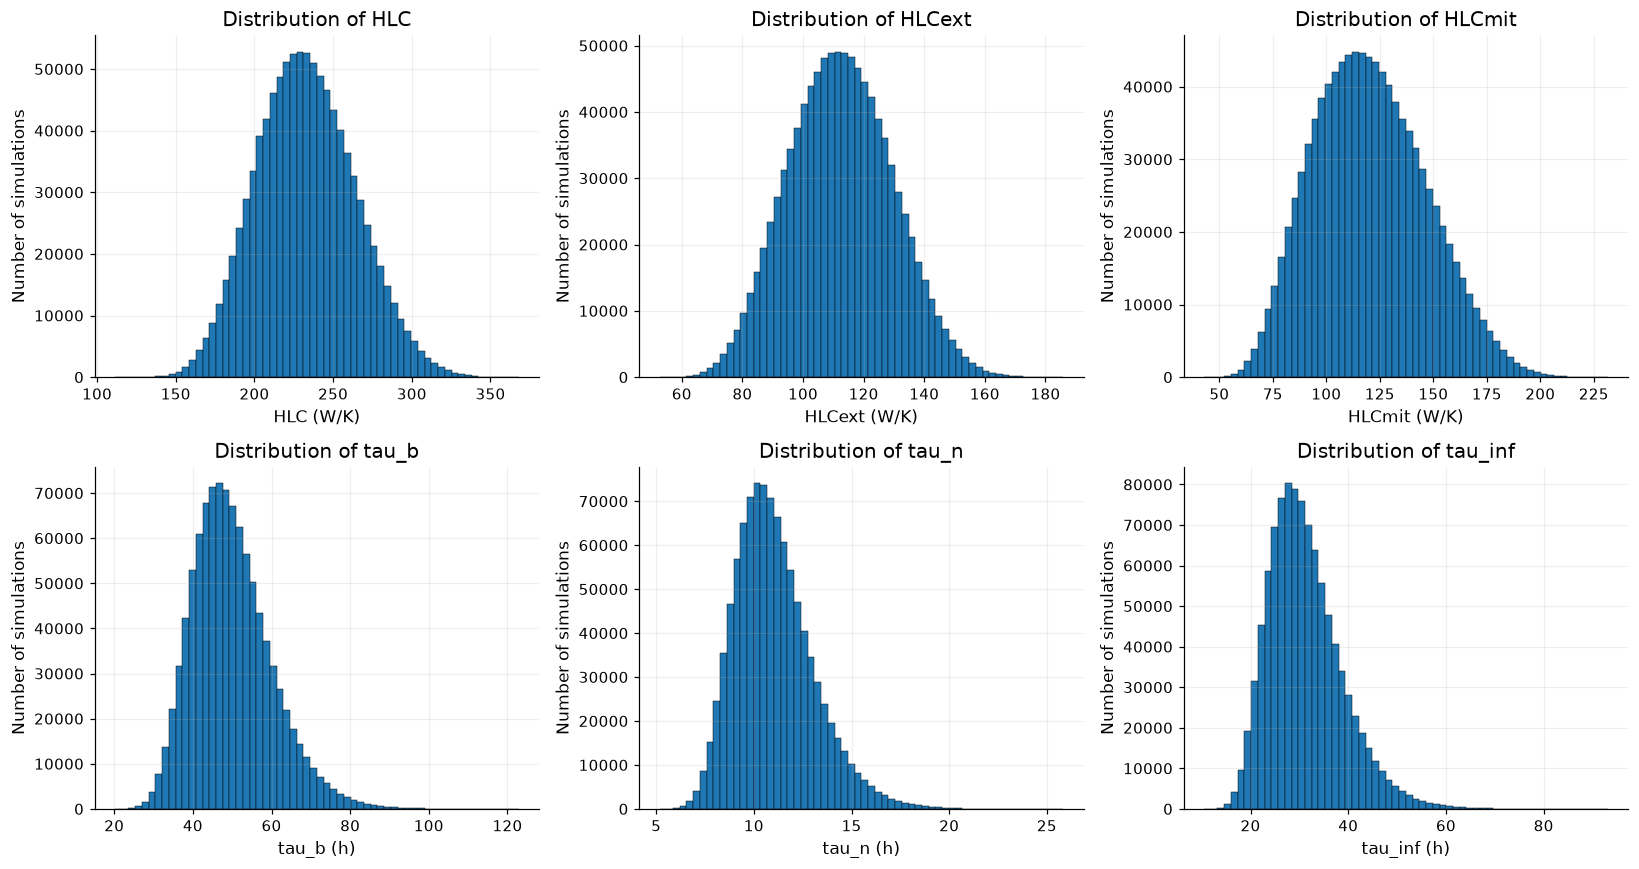
\includegraphics[width=0.92\linewidth]{eda_distributions.png}
\caption{Distributions des six indicateurs thermiques, issues du notebook d'EDA sur un million de simulations.}
\label{fig:eda-distribution}
\end{figure}

J'ai aussi étudié les corrélations entre les paramètres. La corrélation entre $\tau_b$ et $\tau_\infty$ est proche de $0{,}97$ dans les données étudiées. Cette forte association a attiré mon attention : elle peut compliquer l'interprétation des sorties, même si elle ne démontre pas à elle seule une impossibilité de les identifier séparément.

\begin{figure}[htbp]
\centering
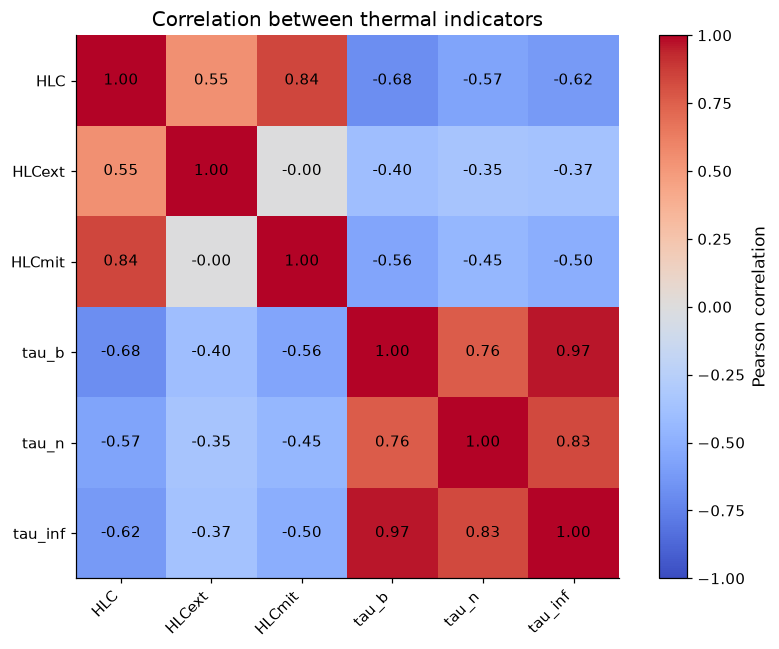
\includegraphics[width=0.69\linewidth]{eda_correlations.png}
\caption{Corrélations empiriques entre les indicateurs, calculées dans le notebook d'EDA.}
\label{fig:eda-correlations}
\end{figure}

\subsection{Nature et diversité des sollicitations}
L'analyse de $U$ a été particulièrement instructive : j'ai compté 907\,125 sollicitations variables, 84\,164 sollicitations nulles et 8\,711 sollicitations constantes non nulles. Bien que le jeu rassemble un million de simulations, il ne contient que \textbf{2\,798 profils $U$ distincts}. Le profil nul apparaît à lui seul 84\,164 fois. Autrement dit, augmenter le nombre de bâtiments simulés ne revient pas à augmenter dans les mêmes proportions la diversité des sollicitations.

\begin{figure}[htbp]
\centering
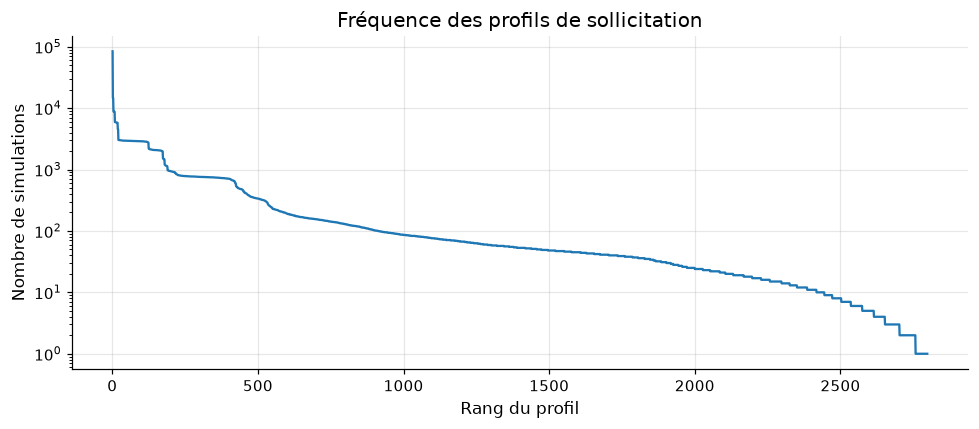
\includegraphics[width=0.90\linewidth]{eda_profils.png}
\caption{Fréquences de répétition des profils de sollicitation $U$ ; de nombreux exemples partagent le même signal d'entrée.}
\label{fig:eda-profils}
\end{figure}

J'ai tenu compte de cette répétition pour construire l'évaluation finale. Le test principal mesure la performance sur des simulations non utilisées à l'entraînement, mais certaines peuvent partager des profils $U$ déjà rencontrés. J'ai donc conservé, en complément, une \textbf{réserve de 287 profils de sollicitation entièrement absents des autres partitions}. Cette réserve permet de tester la généralisation à de nouvelles excitations simulées, sans prétendre garantir une indépendance complète des bâtiments.

\begin{table}[htbp]
\centering
\caption{Répartition fixe de la campagne finale sur 1\,000\,000 simulations.}
\label{tab:split}
\small
\begin{tabular}{lrr}
\toprule
Partition & Nombre de simulations & Part du total \\
\midrule
Entraînement & 719\,885 & 71,99\,\% \\
Validation & 89\,985 & 9,00\,\% \\
Test principal & 89\,987 & 9,00\,\% \\
Réserve U (287 profils non vus) & 100\,143 & 10,01\,\% \\
\bottomrule
\end{tabular}
\end{table}

\FloatBarrier
\section{Prétraitement et définition des entrées}

\subsection{Deux représentations d'une même simulation}
J'ai préparé deux représentations des mêmes données dans \texttt{data\_preprocessing.ipynb}. Pour les réseaux temporels, j'ai conservé les deux signaux complets, sous la forme $(N,2,480)$. Pour le MLP, j'ai extrait \textbf{59 caractéristiques statistiques} : niveaux et dispersions, variations, activité de la sollicitation et résumés sur huit segments temporels. La caractéristique \texttt{T\_initial} étant constante sur l'ensemble d'entraînement, je l'ai supprimée ; il reste donc \textbf{58 caractéristiques}.

Ce choix me permettait de poser une question simple : les résumés statistiques sont-ils suffisants ou les transitions temporelles contiennent-elles une information supplémentaire ? C'est également ce qui m'a conduit, ensuite, à essayer une architecture de fusion.

\subsection{Normalisation calculée sur le train}
J'ai calculé toutes les statistiques de normalisation exclusivement sur les observations d'entraînement, afin d'éviter que le test intervienne dans le choix des transformations. Pour la campagne finale, j'ai utilisé :

\begin{equation}
  T^*=\frac{T-30{,}554748}{4{,}803293},
  \qquad
  U^*=\frac{U}{4791{,}073516}.
  \label{eq:scale}
\end{equation}
J'ai centré et réduit la température. Pour la sollicitation, j'ai préféré une division par sa valeur quadratique moyenne (RMS), \textbf{sans soustraire la moyenne}, pour que l'absence d'excitation ($U=0$) reste représentée par zéro. J'ai standardisé séparément les 58 caractéristiques du MLP en utilisant uniquement leurs statistiques sur le train. Les sorties restent exprimées en unités physiques, tandis que les écarts-types des cibles interviennent dans la fonction de perte.

\begin{figure}[htbp]
\centering
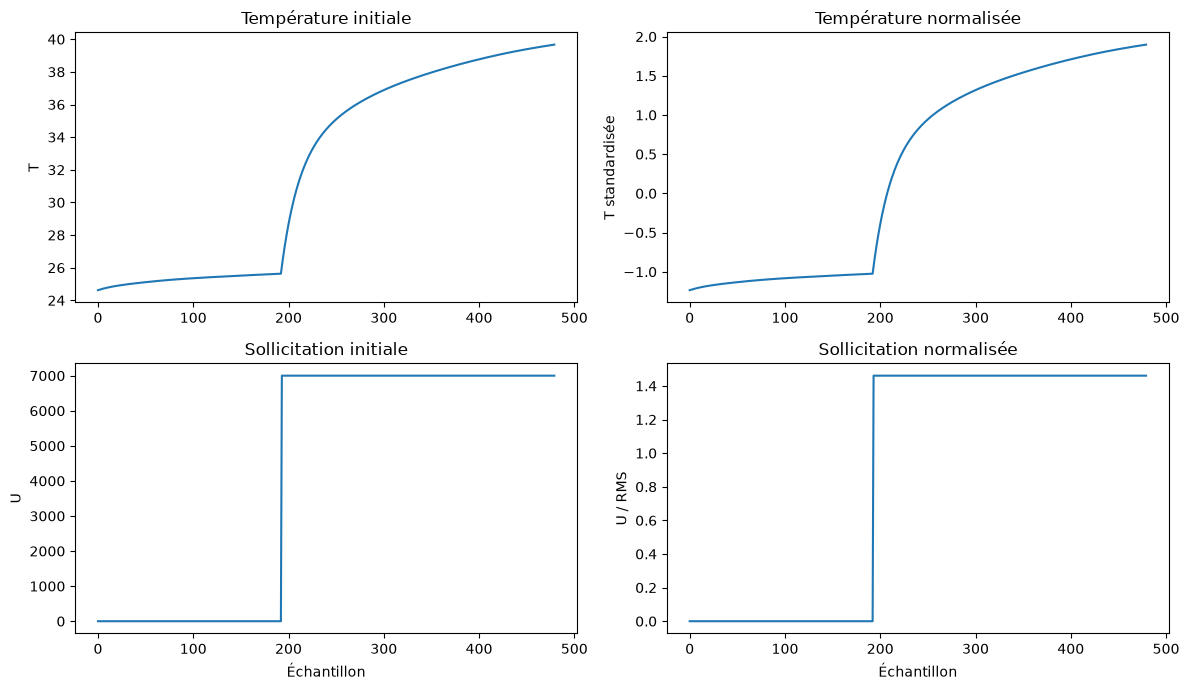
\includegraphics[width=0.78\linewidth]{preprocessing_signaux.png}
\caption{Illustration du changement d'échelle des signaux $T$ et $U$, issue du notebook de prétraitement.}
\label{fig:preprocessing}
\end{figure}

J'ai enregistré les séquences, les caractéristiques, les cibles, les paramètres de normalisation et les partitions afin de réutiliser strictement les mêmes entrées dans les six expériences finales. Les essais préliminaires à 500\,000 simulations avaient leurs propres statistiques de normalisation : je n'ai pas réutilisé celles-ci pour le million.

\subsection{Cinq paramètres indépendants et contrainte physique}
J'ai choisi de faire prédire \textbf{cinq paramètres thermiques indépendants} plutôt que les six paramètres séparément. En effet, la relation $\hlc=\hlcext+\hlcmit$ est déjà connue. Si le réseau prédisait ces trois valeurs indépendamment, rien n'assurerait que leur somme soit cohérente. J'ai donc fait estimer les deux composantes, puis calculé automatiquement le HLC total :

\begin{equation}
 \hat{\boldsymbol y}_{\mathrm{ind}}=(\widehat{\hlcext},\widehat{\hlcmit},\hat\tau_b,\hat\tau_n,\hat\tau_\infty),
 \qquad
 \widehat{\hlc}=\widehat{\hlcext}+\widehat{\hlcmit}.
 \label{eq:physics}
\end{equation}
J'ai utilisé l'activation \emph{Softplus} sur les sorties indépendantes pour obtenir des valeurs positives. Cette construction garantit la cohérence algébrique du HLC, mais pas la précision des prédictions : je calcule donc MAE, RMSE et $R^2$ pour les \emph{six} indicateurs lors de l'évaluation.

Cette décision ne concerne pas cinq \emph{pas temporels futurs}. Les modèles exploitent 480 observations et produisent cinq \emph{paramètres physiques} indépendants. Pour le TCN, le HLC reconstruit est renvoyé directement comme sixième indicateur, tandis que la perte reste calculée sur les cinq paramètres indépendants.

\section{La campagne préliminaire sur 500\,000 simulations}

\subsection{Rôle des essais préliminaires}
Avant d'exploiter le million de simulations, j'ai commencé avec \textbf{500\,000 simulations} pour limiter le coût des premiers essais et comprendre progressivement les modèles. J'ai utilisé 362\,898 observations pour l'entraînement, 45\,361 pour la validation, 45\,365 pour le test principal et 46\,376 pour une réserve de 275 profils $U$ absents du train.

J'ai d'abord testé un MLP avec 60 époques, puis prolongé cette expérience jusqu'à 180 époques. J'ai ensuite essayé un CNN 1D, un CNN--GRU et un TCN. L'objectif n'était pas d'annoncer tout de suite une architecture gagnante, mais de savoir quelles informations semblaient utiles : les statistiques globales, les motifs temporels locaux ou des dépendances plus longues. Les tailles des réseaux et les budgets n'étaient pas tous identiques ; ces essais ont donc joué un rôle d'orientation, plutôt que celui d'une comparaison parfaitement contrôlée.

\begin{table}[htbp]
\centering
\caption{Campagne préliminaire : $R^2$ sur le même test de 45\,365 simulations.}
\label{tab:500k}
\footnotesize
\setlength{\tabcolsep}{4.4pt}
\begin{tabular}{lrrrrr}
\toprule
Cible & MLP 60 & MLP 180 & CNN 1D & CNN--GRU & TCN$^\dagger$ \\
\midrule
HLC & 0,3276 & 0,3474 & 0,3436 & 0,3571 & \textbf{0,3784} \\
HLCext & 0,1373 & 0,1912 & 0,2040 & 0,2974 & \textbf{0,3456} \\
HLCmit & 0,2373 & 0,2387 & 0,2347 & 0,2348 & \textbf{0,2494} \\
$\tau_b$ & 0,0286 & 0,0411 & 0,0462 & 0,0650 & \textbf{0,0813} \\
$\tau_n$ & 0,1605 & 0,1849 & 0,1816 & 0,1984 & \textbf{0,2149} \\
$\tau_\infty$ & 0,0290 & 0,0386 & 0,0420 & 0,0570 & \textbf{0,0687} \\
\bottomrule
\end{tabular}
\vspace{0.2em}
\begin{minipage}{0.99\linewidth}\footnotesize $^\dagger$Les scores TCN préliminaires sont repris du rapport scientifique précédent ; le ZIP préliminaire fourni ne contient pas l'export complet de cette évaluation. Les autres valeurs proviennent des fichiers d'évaluation archivés.\end{minipage}
\end{table}

\subsection{Ce que j'ai retenu des premiers essais}
Les chiffres du tableau~\ref{tab:500k} ont guidé ma progression. Avec le MLP, prolonger l'entraînement de 60 à 180 époques a amélioré HLCext de $0{,}1373$ à $0{,}1912$, mais la prédiction de $\tau_b$ est restée faible ($R^2=0{,}0411$). Le CNN--GRU a nettement amélioré HLCext ($0{,}2974$), ce qui m'a encouragé à utiliser les séries complètes. Dans cette campagne, le TCN a obtenu les meilleurs scores rapportés, notamment $0{,}3456$ pour HLCext, sans résoudre la difficulté de $\tau_b$ ($0{,}0813$) et $\tau_\infty$ ($0{,}0687$).

J'ai donc retenu deux idées à approfondir : enrichir la représentation temporelle du TCN et associer les informations statistiques du MLP aux séquences apprises par le CNN--GRU. Les résultats de cette première étape ne sont pas directement comparables aux scores du million : j'ai gardé les campagnes séparées.

\section{Architectures étudiées et fondements bibliographiques}

\subsection{Du MLP au CNN--GRU et à la fusion}
J'ai commencé par le \textbf{MLP} pour déterminer ce que les 58 caractéristiques construites à partir des signaux pouvaient expliquer. J'ai ensuite utilisé un \textbf{CNN 1D} afin de laisser le réseau apprendre des motifs locaux dans les 480 observations. En passant au \textbf{CNN--GRU}, j'ai ajouté une unité récurrente pour exploiter les relations entre ces motifs au cours du temps.

Enfin, j'ai conçu une \textbf{fusion CNN--GRU + MLP}. La branche temporelle produit 64 caractéristiques apprises, la branche statistique en fournit 32 et je concatène les deux représentations avant la régression. Je voulais vérifier si les résumés statistiques apportaient encore quelque chose aux caractéristiques temporelles. La fusion compte 56\,357 paramètres contre 47\,429 pour le CNN--GRU seul ; j'ai donc gardé à l'esprit qu'un éventuel gain pouvait venir à la fois de la complémentarité des informations et de l'augmentation de capacité.

\subsection{Pourquoi j'ai utilisé SiLU et AdamW}
Dans les couches cachées, j'ai choisi l'activation \textbf{SiLU} (\emph{Sigmoid Linear Unit}), définie par
\begin{equation}
\operatorname{SiLU}(x)=x\,\sigma(x)=\frac{x}{1+e^{-x}}.
\end{equation}
Je l'ai retenue parce qu'elle est \textbf{lisse et dérivable}, contrairement à ReLU qui annule toutes les activations négatives. SiLU laisse passer une partie de l'information dans la région négative et offre une transition progressive entre les régimes d'activation. Ces propriétés la rendaient intéressante pour apprendre des relations non linéaires entre les signaux et les paramètres thermiques. SiLU correspond au cas $\beta=1$ de la famille d'activations \emph{Swish}. \textbf{Je n'ai toutefois pas réalisé d'ablation SiLU/ReLU} : je présente ce choix comme une motivation architecturale, pas comme un gain démontré expérimentalement.

Il est important de distinguer SiLU de \textbf{AdamW}. SiLU transforme les activations \emph{à l'intérieur} du réseau ; \textbf{AdamW est l'optimiseur} qui ajuste ses poids pour réduire la fonction de perte. J'ai utilisé AdamW pour ses pas adaptatifs et sa régularisation \emph{weight decay} découplée de la mise à jour du gradient. Ces deux éléments ont donc des rôles complémentaires, et non interchangeables. J'ai utilisé \emph{Softplus} sur les sorties pour garantir des prédictions positives : c'est encore un troisième rôle, différent de SiLU et d'AdamW.

\subsection{Découverte et fonctionnement du TCN}
Je ne connaissais pas initialement cette architecture. Je l'ai étudiée à partir de l'article de \textbf{Bai, Kolter et Koltun (2018)} \cite{bai2018}, qui montre que des réseaux convolutifs temporels constituent une alternative sérieuse aux modèles récurrents pour plusieurs tâches de séquences. J'ai voulu vérifier cet intérêt sur notre problème inverse, sans supposer que le TCN serait nécessairement meilleur qu'un GRU.

Le principe repose sur des \textbf{convolutions dilatées} : les positions utilisées par un filtre sont espacées de plusieurs pas, ce qui permet d'agrandir le champ réceptif sans multiplier les coefficients du filtre. J'ai également utilisé des \textbf{connexions résiduelles} pour faciliter la circulation des informations à travers les couches empilées. Ces mécanismes font partie des éléments discutés dans la présentation du TCN par Bai et al. \cite{bai2018}.

Dans mon TCN final, j'ai empilé sept blocs résiduels, chacun composé de deux convolutions de noyau 3, avec les dilatations $1,2,4,8,16,32,64$. Le champ réceptif théorique devient :
\begin{equation}
 R=1+2(3-1)\sum_{\ell=0}^{6}2^\ell=509\text{ pas}.
 \label{eq:receptive}
\end{equation}
La portée théorique dépasse ainsi les 480 observations. J'ai aussi ajouté $\Delta T$, $\Delta U$ et six statistiques calculées à partir des signaux. Les convolutions utilisent un \emph{padding} symétrique et sont donc \textbf{non causales} : c'est cohérent ici, puisque je dispose de la séquence complète pour estimer les paramètres, et que je ne réalise pas de prévision en ligne.

\begin{figure}[htbp]
\centering
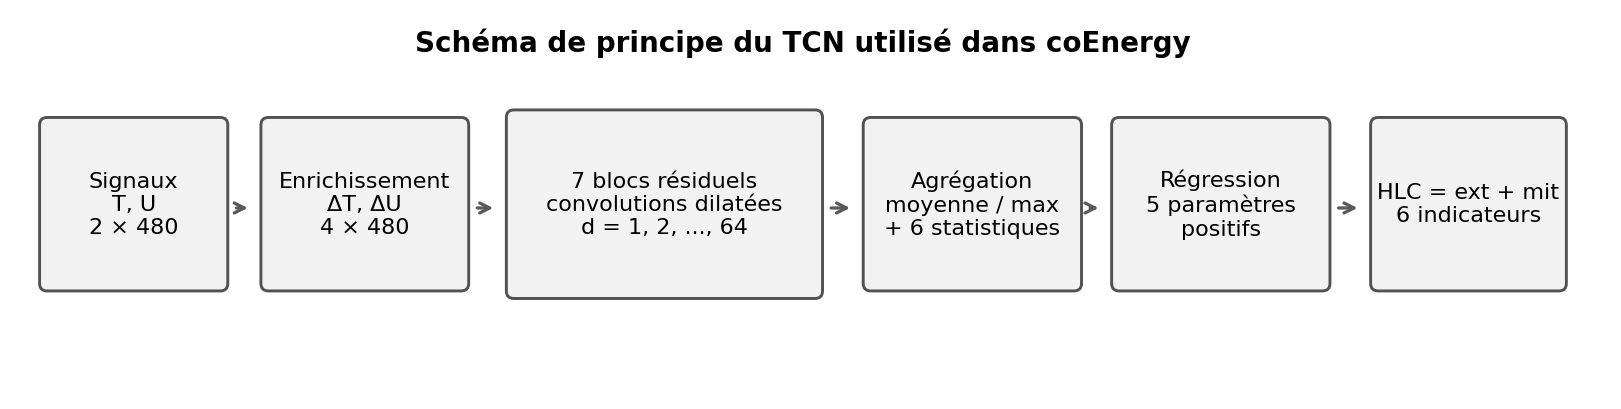
\includegraphics[width=\linewidth]{tcn_architecture.png}
\caption{Schéma fonctionnel du TCN final : enrichissement des signaux, blocs dilatés, agrégation et reconstruction des six indicateurs.}
\label{fig:tcn}
\end{figure}

\subsection{Intérêt et limites du choix TCN}
J'ai retenu le TCN pour trois raisons : un champ réceptif étendu, la possibilité de paralléliser les calculs convolutifs et un nombre de paramètres relativement limité (13\,301 dans ma version finale). Je me suis également appuyé sur une étude liée au projet coEnergy, consacrée à l'identification rapide du HLC à l'aide de simulations, de l'apprentissage automatique et de sollicitations adaptées \cite{coenergy2026}. Ce travail donne un contexte physique à mon approche, mais son objectif principal est l'estimation du HLC global, tandis que j'étudie six indicateurs thermiques.

En contrepartie, un champ réceptif de 509 pas ne prouve pas que le modèle apprend effectivement à utiliser toute la séquence. Le choix des dilatations, la capacité du réseau et le contenu des sollicitations restent déterminants. C'est pour cette raison que j'ai préféré juger le TCN sur ses résultats plutôt que sur ses avantages théoriques.

\section{Protocole de la campagne finale}

\subsection{Entraînement et évaluation}
Pour comparer les configurations finales, j'ai utilisé \textbf{les mêmes 719\,885 simulations d'entraînement}, les mêmes paramètres de normalisation et les mêmes indices de test. J'ai sélectionné les meilleurs poids uniquement sur les 89\,985 observations de validation, puis mesuré les performances sur le test principal et sur la réserve U.

J'ai entraîné les réseaux avec AdamW, une réduction du taux d'apprentissage quand la perte de validation cesse de s'améliorer et un écrêtage des gradients ; sur GPU, j'ai utilisé la précision mixte. Les trois réseaux individuels MLP, CNN 1D et CNN--GRU ont effectué 100 époques, tandis que le TCN et les fusions disposaient d'un maximum de 120 époques, avec arrêt anticipé si la validation ne progressait plus.

\begin{table}[htbp]
\centering
\caption{Dimensions et paramètres des expériences finales (selon les fichiers de configuration archivés).}
\label{tab:hyper}
\small
\begin{tabular}{lrrrl}
\toprule
Modèle & Poids entraînables & Batch & Époques exécutées & Meilleure époque \\
\midrule
MLP             & 9\,509  & 1\,024 & 100 & 100 \\
CNN 1D          & 23\,493 & 1\,024 & 100 & 100 \\
CNN--GRU        & 47\,429 & 1\,024 & 100 & 100 \\
TCN             & 13\,301 & 512 & 113 & 91 \\
Fusion 50/50    & 56\,357 & 1\,024 & 120 & 116 \\
Fusion 30/70    & 56\,357 & 1\,024 & 120 & 114 \\
\bottomrule
\end{tabular}
\end{table}

J'ai défini la \textbf{fonction de perte} sur les cinq grandeurs indépendantes. Comme les paramètres n'ont pas les mêmes unités et amplitudes, je divise chaque erreur par l'écart-type de la cible calculé sur le train. Je calcule ensuite une moyenne d'erreur quadratique pour HLCext/HLCmit et une autre pour les trois constantes de temps :

\begin{equation}
\mathcal{L}_{\alpha}
=\alpha\,\underbrace{\frac12\sum_{j\in\{\mathrm{ext,mit}\}}
\left(\frac{\hat y_j-y_j}{s_j}\right)^2}_{\mathcal{L}_{H}}
+(1-\alpha)\,\underbrace{\frac13\sum_{j\in\{b,n,\infty\}}
\left(\frac{\hat y_j-y_j}{s_j}\right)^2}_{\mathcal{L}_{\tau}}.
\label{eq:loss}
\end{equation}
La moyenne est également prise sur les simulations du mini-batch. Les facteurs $1/2$ et $1/3$ dans l'équation donnent la \emph{moyenne des erreurs à l'intérieur de chaque famille} ; ils ne remplacent pas les poids entre familles. Dans l'expérience de référence, j'ai fixé $\alpha=0{,}5$, soit 50\,\% pour chaque famille. Dans l'expérience \emph{Weighted Loss}, j'ai fixé $\alpha=0{,}3$ pour donner 70\,\% de la perte aux constantes de temps.

\subsection{Indicateurs de performance et cohérence des comparaisons}
J'ai évalué les six paramètres avec la MAE, la RMSE et le coefficient $R^2$. Ce dernier mesure la part de variabilité expliquée par rapport à une prédiction constante égale à la moyenne du jeu évalué :

\begin{equation}
 \mathrm{RMSE}=\sqrt{\frac1N\sum_i(\hat y_i-y_i)^2},\qquad
 R^2=1-\frac{\sum_i(\hat y_i-y_i)^2}{\sum_i(y_i-\bar y)^2}.
\end{equation}
J'ai vérifié que les six archives finales contiennent les checkpoints, les métriques et les prédictions et qu'elles utilisent des empreintes identiques des partitions et du prétraitement. Je peux donc comparer directement leurs scores sur les mêmes observations. En revanche, je ne compare pas directement les \emph{valeurs} des pertes de validation entre les configurations 50/50 et 30/70 : leurs objectifs ne sont pas les mêmes.

\begin{figure}[htbp]
\centering
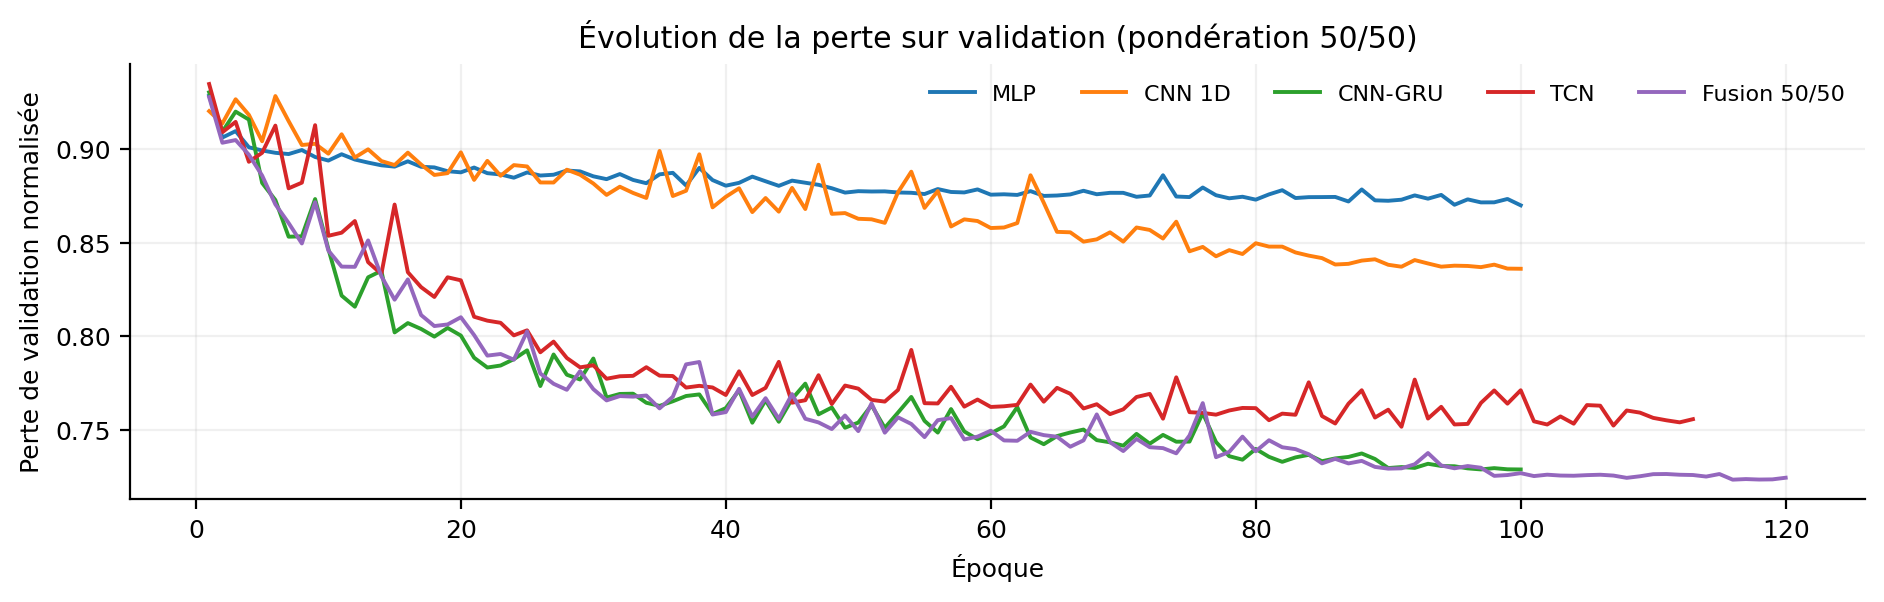
\includegraphics[width=0.91\linewidth]{validation_1m.png}
\caption{Évolution de la perte de validation pour les modèles à pondération 50/50 ; les différentes courbes partagent la même définition de la perte.}
\label{fig:validation}
\end{figure}

\section{Résultats finaux sur un million de simulations}

\subsection{Comparaison sur le test principal}
Le tableau~\ref{tab:final-r2} réunit les valeurs de $R^2$ que j'ai extraites des fichiers \texttt{metrics.csv} des six runs sur les \textbf{89\,987 mêmes simulations de test}. La fusion 50/50 est première sur les six paramètres. Son gain face au CNN--GRU seul est réel dans cette expérience, mais plutôt modeste : $R^2$ progresse de $0{,}4401$ à $0{,}4442$ pour HLC et de $0{,}4815$ à $0{,}4911$ pour HLCext.

\begin{table}[htbp]
\centering
\caption{Campagne finale : coefficients $R^2$ sur le test principal de 89\,987 simulations.}
\label{tab:final-r2}
\footnotesize
\setlength{\tabcolsep}{4.4pt}
\begin{tabular}{lrrrrrr}
\toprule
Cible & MLP & CNN 1D & CNN--GRU & TCN & Fusion 50/50 & Fusion 30/70 \\
\midrule
HLC & 0,3321 & 0,3655 & 0,4401 & 0,4106 & \textbf{0,4442} & 0,4369 \\
HLCext & 0,1442 & 0,2334 & 0,4815 & 0,4342 & \textbf{0,4911} & 0,4805 \\
HLCmit & 0,2420 & 0,2437 & 0,2779 & 0,2676 & \textbf{0,2822} & 0,2771 \\
$\tau_b$ & 0,0343 & 0,0513 & 0,1391 & 0,1262 & \textbf{0,1441} & 0,1397 \\
$\tau_n$ & 0,1693 & 0,2053 & 0,2708 & 0,2539 & \textbf{0,2734} & 0,2691 \\
$\tau_\infty$ & 0,0341 & 0,0475 & 0,1086 & 0,0993 & \textbf{0,1119} & 0,1086 \\
\bottomrule
\end{tabular}
\end{table}

Ce tableau montre ce qui a fonctionné et ce qui reste problématique. L'utilisation directe des séquences a été bénéfique : le MLP atteint seulement $R^2=0{,}1442$ sur HLCext, contre $0{,}4815$ pour le CNN--GRU. La fusion améliore encore ce résultat, mais de seulement $0{,}0096$ point de $R^2$ pour HLCext. Ce gain reste intéressant, sans suffire à prouver que les caractéristiques statistiques, à elles seules, expliquent l'amélioration : la fusion comporte aussi davantage de poids.

En revanche, \textbf{$\tau_b$ et $\tau_\infty$ demeurent difficiles}, même avec le meilleur modèle ($R^2=0{,}1441$ et $0{,}1119$). J'ai donc évité de présenter la fusion comme une solution complète au problème inverse.

\subsection{Précision en unités physiques et réserve U}
J'ai également regardé les erreurs dans les unités physiques. Pour la fusion 50/50, la RMSE vaut \textbf{23,378 W/K pour HLC}, \textbf{12,189 W/K pour HLCext} et \textbf{22,263 W/K pour HLCmit}. Elle atteint \textbf{9,323 h pour $\tau_b$}, \textbf{1,713 h pour $\tau_n$} et \textbf{7,078 h pour $\tau_\infty$}. Je garde ces chiffres en complément de $R^2$, car un coefficient positif n'implique pas automatiquement une erreur faible dans l'unité du paramètre.

J'ai ensuite évalué les mêmes modèles sur les \textbf{100\,143 simulations de réserve U}, correspondant à 287 profils de sollicitation exclus des autres partitions.

\begin{table}[htbp]
\centering
\caption{Coefficients $R^2$ sur la réserve U de 100\,143 simulations (287 profils d'excitation tenus à l'écart).}
\label{tab:reserve}
\footnotesize
\setlength{\tabcolsep}{4.4pt}
\begin{tabular}{lrrrrrr}
\toprule
Cible & MLP & CNN 1D & CNN--GRU & TCN & Fusion 50/50 & Fusion 30/70 \\
\midrule
HLC & 0,3460 & 0,3801 & 0,4422 & 0,4138 & \textbf{0,4462} & 0,4413 \\
HLCext & 0,1350 & 0,2229 & 0,4713 & 0,4301 & \textbf{0,4859} & 0,4786 \\
HLCmit & 0,2517 & 0,2532 & 0,2803 & 0,2695 & \textbf{0,2834} & 0,2806 \\
$\tau_b$ & 0,0313 & 0,0469 & 0,1334 & 0,1239 & \textbf{0,1411} & 0,1375 \\
$\tau_n$ & 0,1641 & 0,1934 & 0,2614 & 0,2468 & \textbf{0,2641} & 0,2622 \\
$\tau_\infty$ & 0,0307 & 0,0419 & 0,1045 & 0,0976 & \textbf{0,1102} & 0,1072 \\
\bottomrule
\end{tabular}
\end{table}

Je n'observe pas d'effondrement des performances sur la réserve U : la fusion 50/50 atteint encore $R^2=0{,}4859$ pour HLCext, $0{,}4462$ pour HLC et $0{,}1411$ pour $\tau_b$. Cette stabilité est encourageante, mais je reste prudent : les répartitions physiques et la difficulté des simulations peuvent différer entre les deux tests. Je n'en déduis donc pas que le modèle est validé sur des bâtiments réels.

\section{Expérience de pondération renforcée : \emph{Weighted Loss}}

\subsection{Pourquoi j'ai essayé la pondération 30/70}
Les premiers essais, puis les résultats finaux, montraient des performances particulièrement faibles sur $\tau_b$ et $\tau_\infty$. J'ai formulé l'hypothèse suivante : \textbf{en donnant plus de poids aux constantes de temps, le réseau pourrait apprendre à mieux les estimer}. J'ai donc repris la même architecture de fusion CNN--GRU + MLP, avec ses 56\,357 paramètres, et remplacé la pondération 50/50 par \textbf{30/70} : 30\,\% pour HLCext/HLCmit et 70\,\% pour les trois constantes de temps.

J'ai conservé les mêmes partitions, la même structure de réseau, la même graine indiquée dans les configurations et les mêmes grandes options d'entraînement. Je pouvais ainsi attribuer la modification principale de cette expérience à la fonction de perte, tout en tenant compte du caractère stochastique de l'optimisation.

\subsection{Ce que j'ai obtenu}
Le résultat a été contraire à mon hypothèse. Sur le test principal, $R^2$ est passé de \textbf{0,1441 à 0,1397} pour $\tau_b$, de \textbf{0,2734 à 0,2691} pour $\tau_n$ et de \textbf{0,1119 à 0,1086} pour $\tau_\infty$. Les trois paramètres HLC ont également obtenu des scores inférieurs. Pour $\tau_b$, la RMSE est passée de 9,323 à 9,347 h ; pour $\tau_\infty$, elle est passée de 7,078 à 7,091 h.

Les écarts sont modestes, mais tous orientés dans le même sens dans ce run : \textbf{la variante 30/70 ne surpasse pas la version 50/50 sur une seule des six cibles}. La réserve U montre la même tendance générale. Je n'ai donc pas retenu cette pondération comme meilleure solution.


\subsection{Comment j'interprète cet échec}
Une première explication possible est qu'\textbf{augmenter le poids de l'erreur ne crée aucune information supplémentaire} dans $T$ et $U$. Si les constantes de temps influencent peu certains segments des signaux ou sont difficiles à distinguer, insister davantage sur leurs erreurs ne permet pas au réseau de retrouver automatiquement la bonne solution.

J'envisage aussi un \textbf{compromis d'optimisation} : les cinq cibles partagent une partie de la représentation apprise, et renforcer une famille peut modifier les gradients sans améliorer la généralisation des autres paramètres. Enfin, le poids optimal peut évoluer pendant l'entraînement ; une pondération fixe de 70\,\% n'est pas nécessairement appropriée à toutes les étapes. La littérature sur les pertes multi-tâches propose, par exemple, des pondérations adaptées à l'incertitude \cite{kendall2018}, que je n'ai pas testées dans ce projet.

Ces explications restent des hypothèses. Pour conclure sur l'effet de la pondération elle-même, il faudrait tester plusieurs valeurs et répéter les entraînements avec différentes graines. \textbf{Mon résultat expérimental est plus limité, mais clair : la configuration 30/70 n'a pas amélioré les scores observés.}

\section{Pourquoi les constantes de temps restent-elles difficiles à estimer ?}

\subsection{Sensibilité temporelle et excitation disponible}
J'ai constaté que les paramètres de déperdition étaient généralement mieux expliqués que les constantes de temps. Une constante de temps caractérise une \emph{dynamique} : pour bien l'estimer, il faut observer une évolution de température suffisamment informative après la sollicitation. Si $U$ reste nul, constant ou peu varié, plusieurs configurations thermiques peuvent conduire à des réponses proches.

Or, mon EDA a montré 84\,164 sollicitations nulles et une forte répétition des profils $U$. Il est donc plausible que certaines simulations renseignent peu sur les dynamiques lentes. L'intérêt de concevoir des sollicitations informatives apparaît également dans l'étude appliquée coEnergy \cite{coenergy2026}. Dans mon cas, je présente cette difficulté comme une hypothèse d'\emph{identifiabilité pratique}, et non comme une impossibilité démontrée. Je ne peux pas non plus vérifier ici que la fenêtre de 480 observations couvre plusieurs fois les constantes de temps les plus grandes, car le pas temporel exact n'est pas suffisamment documenté dans les sources utilisées.

\subsection{Contraction des prédictions vers les valeurs centrales}
J'ai observé dans les nuages de points que les prédictions couvrent souvent une plage bien plus étroite que les vraies valeurs. Pour la meilleure fusion 50/50, l'écart-type des prédictions ne représente qu'environ \textbf{39,5\,\%} de l'écart-type réel pour $\tau_b$, \textbf{52,8\,\%} pour $\tau_n$ et \textbf{35,0\,\%} pour $\tau_\infty$.

Ce phénomène de \textbf{sous-dispersion} m'aide à comprendre les faibles $R^2$ : les petites constantes de temps tendent à être surestimées et les grandes à être sous-estimées. En minimisant l'erreur quadratique, le réseau peut converger vers des valeurs proches de la moyenne conditionnelle lorsque les entrées ne permettent pas de distinguer clairement les cas. Le nuage de points de la figure~\ref{fig:scatter} rend cette limite visible sans avoir besoin d'un graphique supplémentaire de ratios.

\begin{figure}[htbp]
\centering
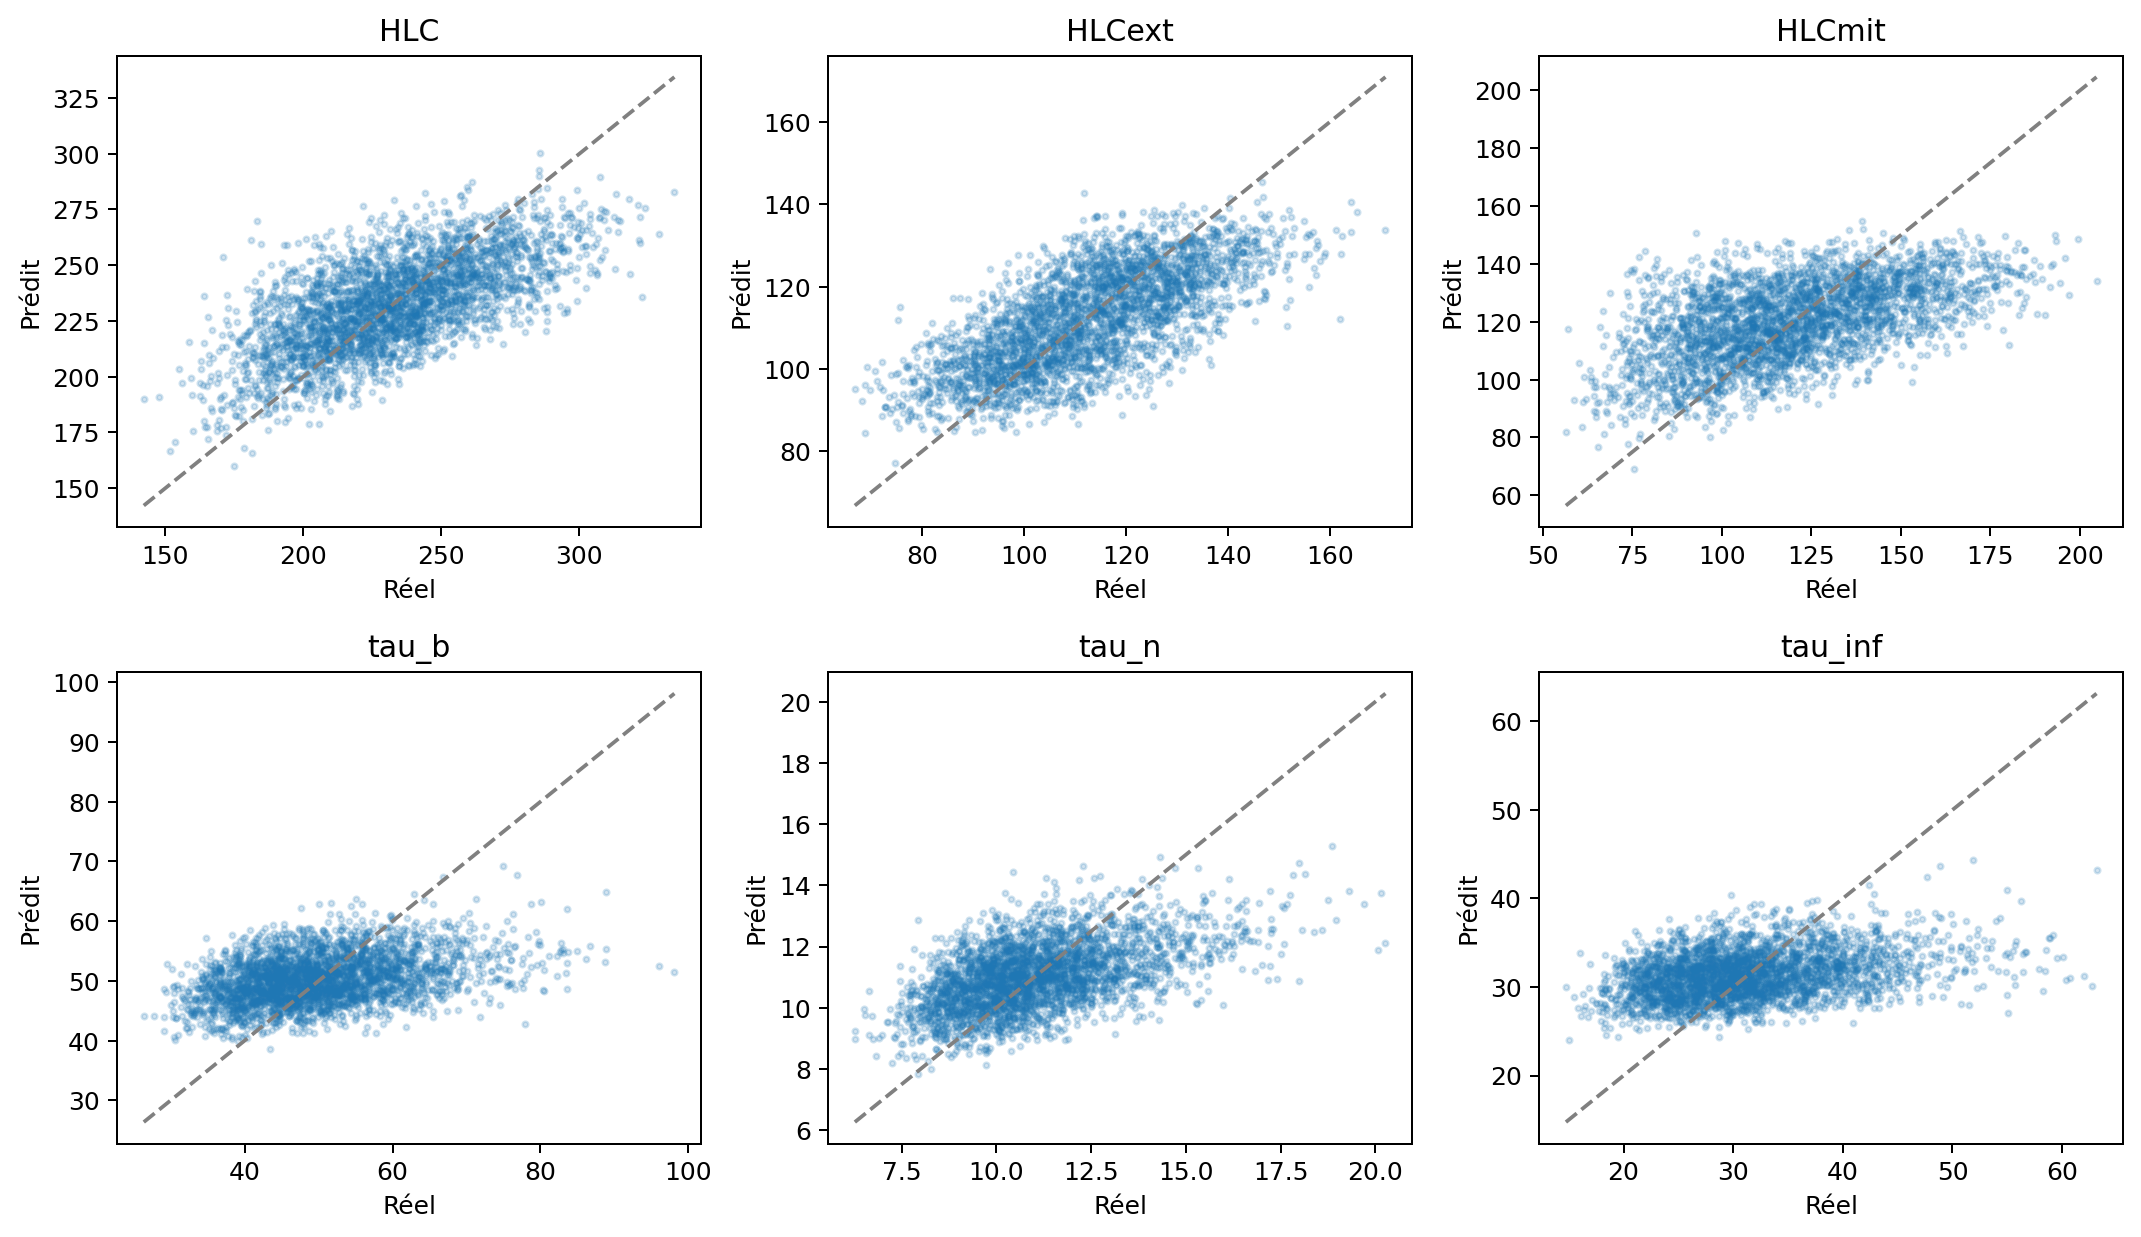
\includegraphics[width=0.92\linewidth]{scatter_fusion_50_50.png}
\caption{Valeurs réelles et prédites pour la fusion 50/50 sur le test principal (échantillon de visualisation) ; la diagonale correspond à la prédiction parfaite.}
\label{fig:scatter}
\end{figure}

\subsection{Variabilité, corrélations et limites des données simulées}
Les distributions des constantes de temps sont asymétriques et leurs corrélations sont parfois fortes. J'ai donc envisagé trois causes possibles des erreurs : une sollicitation qui révèle insuffisamment certaines propriétés, une ambiguïté entre configurations produisant des réponses similaires et une capacité limitée des modèles à exploiter les informations disponibles.

Je ne peux pas départager ces explications avec les seuls scores. En outre, mes données sont simulées : je n'ai pas mesuré l'effet d'un bruit instrumental réel ni validé les prédictions sur un bâtiment physique. Ces limites doivent être prises en compte avant toute généralisation au terrain.

\section{Discussion générale et conclusion}
Je retiens d'abord que \textbf{l'information temporelle compte}. Sur le test final, le passage du MLP au CNN--GRU fait progresser HLCext de $R^2=0{,}1442$ à $0{,}4815$. La fusion 50/50 va un peu plus loin ($0{,}4911$), mais son avantage reste modéré et doit être nuancé par son nombre supérieur de paramètres. Le CNN--GRU individuel apparaît donc comme une alternative intéressante si je privilégie une architecture un peu plus légère.

Les essais préliminaires m'avaient conduit à considérer le TCN comme une piste prometteuse. Sur un million de simulations, la version finale est toutefois dépassée par le CNN--GRU et par la fusion 50/50 sur les six cibles. Je n'y vois pas une remise en cause du principe des convolutions dilatées : j'ai changé la quantité de données, certaines dimensions architecturales et les budgets d'entraînement. C'est précisément pour éviter une comparaison trompeuse que j'ai conservé les résultats préliminaires séparés.

J'ai aussi testé une \textbf{Weighted Loss 30/70} pour mieux prédire les constantes de temps. Elle n'a pas apporté le gain attendu, ce qui m'a montré qu'une modification de l'objectif ne suffit pas toujours à résoudre une difficulté provenant peut-être de l'information contenue dans les signaux. La sous-dispersion de $\tau_b$ et de $\tau_\infty$ constitue, à mon avis, le principal résultat à approfondir.

Pour aller plus loin, je pourrais tester plusieurs graines aléatoires, comparer les modèles à capacité égale et étudier de nouvelles sollicitations ainsi que l'incertitude des prédictions. En l'état, \textbf{je retiens la fusion CNN--GRU + MLP 50/50 comme meilleur modèle observé}, tout en considérant que la précision des constantes de temps reste insuffisante et que les données simulées limitent la portée des conclusions. J'ai enfin imposé la relation $\hlc=\hlcext+\hlcmit$ par construction, ce qui assure une cohérence physique simple pour l'ensemble des modèles.

\small
\begin{thebibliography}{3}
\bibitem{bai2018} S. Bai, J. Z. Kolter et V. Koltun (2018).
\emph{An Empirical Evaluation of Generic Convolutional and Recurrent Networks for Sequence Modeling}.
arXiv:1803.01271. \url{https://arxiv.org/abs/1803.01271}.

\bibitem{coenergy2026} R. Nassif, S. Guernouti, P. Stabat et M. Cohen (2026).
\emph{Building-specific excitation optimization and simulation-driven machine learning for rapid in situ identification of the heat loss coefficient}.
Prépublication SSRN 6928008. \url{https://doi.org/10.2139/ssrn.6928008}.

\bibitem{kendall2018} A. Kendall, Y. Gal et R. Cipolla (2018).
\emph{Multi-Task Learning Using Uncertainty to Weigh Losses for Scene Geometry and Semantics}.
Proceedings of CVPR. \url{https://doi.org/10.1109/CVPR.2018.00781}.
\end{thebibliography}

\end{document}
